% ACIIDS 2027 submission -- LNCS/LNAI, 12--15 pages incl. references (CFP).
% Structure mirrors the ACIIDS 2026 AutoViVQA paper (refs:autovqa/): main.tex +
% Section/*.tex + splncs04.
%
% NUMBERS: all tables and figures use the whole-image re-evaluation
% (exp/eval-input-diagnostic, plans/paper-tables-full-image.md, 2026-10-05);
% Full Q-Former is the leak-fixed retrain (4a8eb6d). Old crop / leaky numbers: none.

\documentclass[runningheads]{llncs}
\usepackage[T1]{fontenc}
\usepackage[utf8]{inputenc}
\usepackage{graphicx}
\usepackage{url}
\usepackage{booktabs}
\usepackage{amsmath}
\usepackage{amssymb}
\usepackage{multirow}
\usepackage{xcolor}
\usepackage{microtype}
\usepackage{tikz}
\usetikzlibrary{positioning,arrows.meta,fit}
\usepackage[hidelinks]{hyperref}
\usepackage{caption}
\captionsetup{labelfont=bf}

\graphicspath{{figures/}}

\setlength{\textfloatsep}{8pt plus 2pt minus 2pt}
\setlength{\intextsep}{8pt plus 2pt minus 2pt}
\setlength{\abovecaptionskip}{4pt}

% Set to 0 for the submission build: hides every \todo{}.
\newif\ifshowtodo \showtodotrue
\newcommand{\todo}[1]{\ifshowtodo\textcolor{red}{[TODO: #1]}\fi}
\newcommand{\dF}{$\Delta$F1}
% corresponding-author envelope, as in the ACIIDS 2026 paper
\newcommand{\mygraphic}[1]{
\includegraphics[height=#1]{drawing.pdf}}
\newcommand{\myenv}{(\raisebox{0pt}{\mygraphic{.6em}})}
\newcommand{\myauthor}[1]{#1~\myenv}
\newcommand\blfootnote[1]{\begingroup\renewcommand\thefootnote{}\footnote{#1}\addtocounter{footnote}{-1}\endgroup}
% OOD study: \oodtexttrue = 4 datasets (incl. scene-text ViTextVQA/OpenViVQA);
% \oodtextfalse = only the 2 general-domain datasets (ViVQA-X, ViVQA).
% Decide after the whole-image OOD re-evaluation (ood-full jobs).
\newif\ifoodtext \oodtextfalse

\begin{document}

% Named after the group's series: AutoViVQA (ACIIDS 2026) -> ViMoE-VQA -> ViBridge-VQA.
% Earlier candidates: "Decoder, Not Vision: ..." (dropped: OOD scene-text result shows the
% vision side matters), "Look Once, Tune the Decoder: ...".
\title{ViBridge-VQA: Parameter-Efficient Adaptation of a Frozen Vision--Language Model for Vietnamese Visual Question Answering}
\titlerunning{ViBridge-VQA: Parameter-Efficient Adaptation for Vietnamese VQA}

% Author block taken from the ACIIDS 2026 AutoViVQA paper, first author moved to the front.
\author{
Nguyen~Trung~Quoc\orcidID{0009-0009-4569-3932} \and
Nguyen~Anh~Tuong\orcidID{0009-0002-3457-5745} \and
Phan~Ba~Duc\orcidID{0009-0000-1816-9224} \and
Tran~Dac~Thinh\orcidID{0009-0007-8187-4605} \and
Dang~Duy~Lan\orcidID{0009-0007-8658-6602} \and
Nguyen~Quoc~Thinh\orcidID{0009-0001-6765-1276} \and
\myauthor{Tung~Le}\orcidID{0000-0002-9900-7047}
}
\authorrunning{N. T. Quoc et al.}
\institute{
Faculty of Information Technology, University of Science, Ho Chi Minh City, Vietnam\\
Vietnam National University, Ho Chi Minh City, Vietnam\\
\email{\{22120071,22120182,22120301,22120347,}\\
\email{22120348,22120412\}@student.hcmus.edu.vn, lttung@fit.hcmus.edu.vn}
\blfootnote{\myenv{}Corresponding author: Tung Le -- lttung@fit.hcmus.edu.vn}
}

\maketitle

\begin{abstract}
Vision--language models (VLMs) have advanced Visual Question Answering (VQA)
substantially, yet adapting them to a new Vietnamese benchmark usually means
fine-tuning on high-resolution multi-tile inputs or designing a new architecture.
We propose \textbf{ViBridge-VQA}, a parameter-efficient method that improves the
Vietnamese VLM Vintern-1B for generative VQA at a fraction of its cost. ViBridge-VQA
keeps both pre-trained backbones frozen, replaces the projector with a lightweight
multi-token bridge, and trains it jointly with a rank-16 decoder LoRA, so that only
1.01\% of the parameters are trained and each image is encoded as a single view. On
AutoViVQA, ViBridge-VQA raises the token F1 of Vintern-1B from 17.6 to 54.5 and its
CIDEr from 8.5 to 108.4. It outperforms the officially fine-tuned Vintern-1B on
seven of eight metrics, including F1 (+0.8), BLEU (+14.9), METEOR (+9.8) and CIDEr
(+35.6), while encoding up to six times fewer image tiles, and it achieves the best
BLEU, ROUGE-L, METEOR and CIDEr among all compared systems. A component-wise
analysis shows that adapting the decoder is the key ingredient: it improves every
bridge design and reduces their F1 spread from 5.6 to 0.8 points, whereas larger
bridges and representation alignment do not help. ViBridge-VQA benefits most on
reasoning-intensive questions and also transfers to other Vietnamese VQA datasets.

\keywords{Vietnamese Visual Question Answering \and Vision--Language Models \and
Parameter-Efficient Fine-Tuning \and Low-Rank Adaptation \and Generative VQA}
\end{abstract}

\section{Introduction}
\label{sec:intro}

Visual Question Answering (VQA) asks a model to answer a natural-language question
about an image, which requires it to perceive the visual content, understand the
question and reason over both. The task has progressed rapidly with large
vision--language models (VLMs) such as BLIP-2~\cite{li2023blip2},
Flamingo~\cite{alayrac2022flamingo} and LLaVA~\cite{liu2023visualinstructiontuning},
which connect a pre-trained vision encoder to a pre-trained language model and
generate free-form answers. Vietnamese has followed this trend: Vintern-1B~\cite{doan2024vintern1b}
connects an InternViT-300M encoder~\cite{chen2024internvl} to a Qwen2.5-0.5B
decoder~\cite{qwen2025qwen25} and is among the strongest open Vietnamese VLMs, while
benchmarks such as ViVQA~\cite{tran2021vivqa}, OpenViVQA~\cite{nguyen2023openvivqa} and
the recent reasoning-oriented AutoViVQA~\cite{autovivqa2026} make it possible to measure
progress in this low-resource setting.

Obtaining a strong model on a new Vietnamese benchmark, however, is still expensive.
The common recipe fine-tunes an existing VLM: the fine-tuned Vintern-1B baseline of
AutoViVQA adds LoRA adapters to the language model and splits every image into up to
six high-resolution tiles plus a thumbnail, so that the decoder reads up to 1{,}792
visual tokens per image. The alternative is to design a task-specific architecture, as
ViMoE-VQA~\cite{vimoevqa} does with a sparse mixture-of-experts fusion module and a
decoder trained on AutoViVQA. A cheaper option is to keep the whole VLM frozen and train
only a small connector between its encoder and decoder, but the design of that
connector is delicate. A connector that reads only the global image vector is light,
yet it cannot convey small objects, printed text or spatial relations. Connectors that
learn to compress the patch tokens, such as Q-Formers, can convey such details but
must learn a new alignment to the decoder from limited Vietnamese data.

Vintern-1B already contains a component that solves this alignment problem: its
projector, which was pre-trained to map image regions into the input space of the
decoder. At the same time, it discards the global \texttt{[CLS]} vector of its encoder,
which summarises the whole scene. This observation raises a simple question:
\emph{which visual tokens should a frozen Vietnamese VLM receive, and how many?}

To address this question, we propose \textbf{ViBridge-VQA}, which gives the frozen
decoder of Vintern-1B two complementary kinds of visual tokens from a single image view.
\emph{Local} tokens reuse the frozen projector of Vintern-1B, average-pooled to a chosen
budget and placed in its original image slot, so the decoder receives region features
in the representation it was trained to read. \emph{Global} tokens are produced from the
\texttt{[CLS]} vector by a small trainable bridge and add the scene-level information that
Vintern-1B ignores. Only this bridge is trained. Because every additional token
increases inference cost, we treat the number of global and local tokens as a budget
and select it as the knee of the accuracy--cost Pareto front. As a result, ViBridge-VQA
with 14 global and 36 local tokens outperforms the officially fine-tuned Vintern-1B on most metrics while reading up to 36 times fewer visual tokens and updating none of its weights.

In summary, our main contributions are as follows:
\begin{itemize}
  \item We propose \textbf{ViBridge-VQA}, a global--local bridge that improves a frozen
  Vietnamese VLM by combining trainable global tokens with local tokens from its own
  pre-trained projector. It raises the F1 of Vintern-1B on AutoViVQA from 17.6
  (zero-shot) to 54.6 with 1.35\% of the parameters trained, and to 58.2 when combined
  with a lightweight decoder LoRA.
  \item We study the \textbf{visual token budget} systematically over eight
  configurations and three random seeds, and select it with an explicit criterion. The
  knee of the Pareto front falls on the same configuration for every metric, on both
  evaluation splits, and for cost measured in tokens or in inference time.
  \item We \textbf{analyse where the gains come from}: local tokens matter far more than
  global ones, should come from the pre-trained projector, complement decoder
  adaptation, and transfer to four unseen Vietnamese VQA datasets.
\end{itemize}

\section{Related Work}
\label{sec:related}

Early VQA systems classified over a fixed set of answers, whereas current generative VLMs produce free-form answers with an autoregressive language
model~\cite{li2023blip2,alayrac2022flamingo,liu2023visualinstructiontuning}. Vietnamese datasets include ViVQA~\cite{tran2021vivqa}, OpenViVQA~\cite{nguyen2023openvivqa},
ViCLEVR~\cite{tran2023viclevr}, ViOCRVQA~\cite{pham2024viocrvqa} and ViTextVQA~\cite{nguyen2025vitextvqa}. AutoViVQA~\cite{autovivqa2026} contributes 37{,}077
questions on 19{,}411 COCO images~\cite{lin2015coco}, generated by large language models,
filtered by an ensemble of validators and annotated with reasoning categories, with an
emphasis on relational, causal and multi-step reasoning. On the modelling side,
BARTPhoBEiT~\cite{tran2023bartphobeitpretrainedsequencetosequenceimage} and
AViVQA-TranConI~\cite{nguyen2024tranconi} combine pre-trained visual and Vietnamese
language representations, Vintern-1B~\cite{doan2024vintern1b} brings an instruction-tuned
VLM to Vietnamese, and ViMoE-VQA~\cite{vimoevqa} routes multimodal tokens to sparse experts
for generative VQA on AutoViVQA. These approaches either train a new model or fine-tune an
existing VLM on multi-tile inputs; in contrast, we keep every pre-trained weight of
Vintern-1B frozen and use a single image view.

Keeping the vision encoder and the language model frozen and training only a connector is a
common way to build VLMs efficiently, and connectors differ mainly in what they must learn.
Frozen~\cite{tsimpoukelli2021frozen} learns a visual prefix from a global image
representation. The Q-Former of BLIP-2~\cite{li2023blip2} learns a set of queries that
compress the patch features, which preserves details but requires a large module (188M
parameters) pre-trained on millions of image--text pairs. LLaVA~\cite{liu2023visualinstructiontuning,liu2024llava15}
projects every patch token with a small MLP, which preserves locality but passes hundreds of
tokens to the decoder; Honeybee~\cite{cha2024honeybee} proposes locality-preserving
abstractors, and InternVL~\cite{chen2024internvl}, on which Vintern-1B is built, merges
neighbouring patches before its MLP projector. In all of these models, the mapping from
patches to the decoder is learned during large-scale pre-training. ViBridge-VQA differs in two
respects: it does not learn this local mapping again but reuses the projector already
pre-trained in the VLM, and it trains only a small global bridge (12.9M parameters) on about
26k task questions. 

The number of visual tokens largely determines the cost of the decoder. Inference-optimal
scaling of VLMs~\cite{li2024inferenceoptimal} shows that a few tokens can suffice for many
tasks, and Matryoshka multimodal models~\cite{cai2024matryoshka} train a model to work at
several nested pooled token budgets and show that the required budget depends on the task.
These approaches train or re-train the model for each budget. In contrast, we keep the model
frozen and obtain each budget simply by pooling the output of the frozen projector, and we
choose among budgets with explicit criteria, namely the knee of the Pareto
front~\cite{satopaa2011kneedle} and TOPSIS~\cite{hwang1981topsis}. Parameter-efficient
methods such as adapters~\cite{houlsby2019adapters}, prefix tuning~\cite{li2021prefix} and
LoRA~\cite{hu2022lora} reduce the cost of adaptation from the other side, by training a small
number of additional weights in the decoder. We use decoder LoRA both as a baseline and as a
complement, and ask whether a small training budget is better spent on the visual tokens or on
adapting the decoder.

\section{Proposed Method}
\label{sec:method}

We formulate VQA as conditional answer generation: given an image $I$ and a Vietnamese
question $q$, the model generates a short free-form answer $y=(y_1,\dots,y_T)$.
ViBridge-VQA builds on Vintern-1B~\cite{doan2024vintern1b} and keeps all of its
pre-trained weights frozen. Instead of adapting the model, it changes what the decoder sees. 

\begin{figure}[t]
\centering
\resizebox{\linewidth}{!}{%
\begin{tikzpicture}[font=\small, node distance=3.5mm,
  frozen/.style={draw=gray!70, rounded corners=2pt, fill=gray!10, minimum height=9mm, align=center},
  train/.style={draw=green!45!black, rounded corners=2pt, fill=green!12, thick, minimum height=9mm, align=center},
  data/.style={align=center, text=black!75},
  arr/.style={-{Latex[length=1.6mm]}, thick, black!70},
  lbl/.style={font=\footnotesize\bfseries, anchor=west}]
% ---- row 1: official fine-tuning of Vintern-1B
\node[lbl] (t1) at (0,1.2) {(a) Vintern-1B, official fine-tuning};
\node[data] (img1) at (0.7,0) {image\\$\le$6 tiles + thumbnail\\($448^2$ each)};
\node[frozen, right=of img1] (vit1) {InternViT-300M};
\node[frozen, right=of vit1] (mlp1) {projector\\(patches, $2{\times}2$ merge)};
\node[data, right=of mlp1] (tok1) {256 tokens / tile\\($\le$1{,}792)};
\node[frozen, right=of tok1, text width=27mm] (llm1) {Qwen2.5-0.5B\\+ \textcolor{green!45!black}{\textbf{LoRA} $r{=}16$}};
\node[data, right=of llm1] (ans1) {answer};
\draw[arr] (img1) -- (vit1); \draw[arr] (vit1) -- (mlp1); \draw[arr] (mlp1) -- (tok1);
\draw[arr] (tok1) -- (llm1); \draw[arr] (llm1) -- (ans1);
% ---- row 2: ViBridge-VQA
\node[lbl] (t2) at (0,-1.5) {(b) ViBridge-VQA (ours)};
\node[data] (img2) at (0.7,-3.1) {image\\1 view\\($336^2$)};
\node[frozen] (vit2) at (vit1 |- img2) {InternViT-300M};
\node[train] (br) at ($(mlp1 |- img2)+(0,0.75)$) {\textbf{global bridge}\\(\texttt{[CLS]} $\to g$ tokens)};
\node[frozen] (pj) at ($(mlp1 |- img2)+(0,-0.75)$) {projector of Vintern-1B\\+ avg.\ pool to $k$};
\node[data] (tg) at (tok1 |- br) {$g$ global tokens\\(prefix)};
\node[data] (tl) at (tok1 |- pj) {$k$ local tokens\\(image slot)};
\node[frozen, text width=27mm] (llm2) at (llm1 |- img2) {Qwen2.5-0.5B\\(frozen, no LoRA)};
\node[data, right=of llm2] (ans2) {answer};
\draw[arr] (img2) -- (vit2);
\draw[arr] (vit2.east) -- ++(0.15,0) |- (br.west);
\draw[arr] (vit2.east) -- ++(0.15,0) |- (pj.west);
\draw[arr] (br) -- (tg); \draw[arr] (pj) -- (tl);
\draw[arr] (tg.east) -- ++(0.15,0) |- (llm2.west);
\draw[arr] (tl.east) -- ++(0.15,0) |- (llm2.west);
\draw[arr] (llm2) -- (ans2);
% legend
\node[frozen, minimum height=4mm, minimum width=5mm] (lf) at (13.2,-4.6) {};
\node[anchor=west] at (lf.east) {frozen};
\node[train, minimum height=4mm, minimum width=5mm] (lt) at (15.0,-4.6) {};
\node[anchor=west] at (lt.east) {trained};
\end{tikzpicture}}
\caption{Overview of ViBridge-VQA compared with the official fine-tuning of Vintern-1B.
(a) The official recipe encodes up to seven views per image, passes up to 1{,}792 visual
tokens to the decoder and adapts the decoder with LoRA. (b) ViBridge-VQA encodes a single
view and passes $g$ global tokens, produced from the \texttt{[CLS]} vector by a trainable
bridge, and $k$ local tokens, produced by the frozen projector of Vintern-1B and
average-pooled. Only the global bridge is trained (1.35\% of the parameters for
$g=14$); the selected budget is $g=14$, $k=36$.}
\label{fig:arch}
\end{figure}

\subsection{Overall Architecture}
\label{sec:encoding}

As illustrated in Fig.~\ref{fig:arch}, ViBridge-VQA keeps the three components of
Vintern-1B: the InternViT-300M vision encoder (24 layers, width 1024), its two-layer MLP
projector $P$, and the Qwen2.5-0.5B-Instruct language decoder (24 layers, width 896).
Each image is resized to one $336\times336$ view ($24\times24$ patches of $14\times14$ pixels);
the encoder returns one vector per patch and a global \texttt{[CLS]} vector $v\in\mathbb{R}^{1024}$.
Vintern-1B uses only the patch vectors: it merges every $2\times2$ block of neighbouring
patches into one 4096-dimensional vector (pixel shuffle) and maps each merged vector into
the decoder input space with $P$, which was pre-trained to align the two backbones. At our
resolution this yields a $12\times12$ grid of 144 region tokens. ViBridge-VQA uses both outputs of the encoder.

\subsection{Global Tokens}
\label{sec:bridge}

The \texttt{[CLS]} vector summarises the whole scene, but Vintern-1B never passes it to
the decoder. A small trainable bridge $g_\phi$ expands it into $g$ tokens with two linear
heads:
\begin{equation}
  g_\phi(v) = \big[\,W_a v + b_a;\ \mathrm{reshape}_{(g-1)\times 896}(W_e v + b_e)\,\big]
  \in \mathbb{R}^{g\times 896}.
  \label{eq:bridge}
\end{equation}
where $W_a\in\mathbb{R}^{896\times1024}$ and $W_e\in\mathbb{R}^{(g-1)896\times1024}$. The first
head produces an \emph{anchor} token, and the second produces $g-1$ complementary tokens that
present the global content to the decoder from different learned directions. The bridge has
$1025\cdot896\cdot g$ parameters, i.e., 12{,}857{,}600 for $g=14$, and its $g$ tokens are
placed before the prompt. We use $g=14$ because, in a preliminary study, the F1 of this bridge
alone rose with $g$ up to 14 and then plateaued.

\subsection{Local Tokens}
\label{sec:local}

Global tokens alone cannot describe small objects, printed text or the position of
objects. ViBridge-VQA therefore also passes local tokens, taken directly from the 144
region tokens of the frozen projector $P$. To control their number, we average-pool the
$12\times12$ grid to an $s\times s$ grid, so that $k=s^2$ with $s\in\{1,3,6,12\}$: $k=144$
keeps every region token, and $k=36$ averages each $2\times2$ block. The pooled tokens
replace the embeddings of $k$ image-context placeholders inside Vintern-1B's own image
slot, \texttt{<img>}\,$\cdots$\,\texttt{</img>}, in the prompt. Because they come from the
pre-trained projector rather than from a newly learned projection of the patches, the
local tokens stay in the representation that the decoder was trained to read, and no
parameters are needed to produce them.

\subsection{Training Objective}
\label{sec:training}

Only the bridge parameters $\phi$ are trained; the vision encoder, the projector and the
decoder remain frozen, and no adapter is added to the decoder. We minimise the
cross-entropy of the answer tokens:
\begin{equation}
  \mathcal{L} = -\sum_{t=1}^{T} \log p\big(y_t \mid y_{<t},\, g_\phi(v),\, \mathrm{pool}_s(P(x)),\, q\big),
  \label{eq:ce}
\end{equation}
where $x$ denotes the merged patch vectors. ViBridge-VQA can also be combined with decoder adaptation: in that variant, a rank-16
LoRA~\cite{hu2022lora} on the query, key, value and output projections of every decoder layer is
trained jointly with the bridge, which adds 2{,}162{,}688 parameters. Throughout the paper,
percentages of trained parameters are relative to all parameters of the model, i.e., the
frozen components of Vintern-1B (about 0.94B, including the vision encoder, projector,
embeddings and output layer) plus the trained modules. With $g=14$, the bridge alone trains
12.86M parameters (1.35\%), and the bridge with LoRA 15.02M (1.57\%).

\subsection{Choosing the Token Budget}
\label{sec:budget}

The cost of the decoder grows with the number of visual tokens $g+k$, so we treat the pair
$(g,k)$ as a budget to be chosen. In our experiments, accuracy increases monotonically
with the number of visual tokens, so every configuration lies on the accuracy--cost Pareto front and
the front alone does not single one out. We therefore select its
\emph{knee}~\cite{satopaa2011kneedle}, the point after which additional tokens bring
diminishing returns. After normalising cost $c$ and accuracy $a$ to $[0,1]$ over the front,
the knee is the configuration that maximises $\hat a - \hat c$, i.e., the one lying
furthest above the line joining the cheapest and the most accurate configuration. The knee is computed on the validation split only, and we check the choice with the
multi-criteria method TOPSIS~\cite{hwang1981topsis}, also on validation, under several
weightings of accuracy and cost. Test results are computed for every configuration only to be
reported; no choice is based on them.

\section{Experiments}
\label{sec:exp}

We evaluate how much ViBridge-VQA improves Vintern-1B, how many tokens it should use,
where its gains come from, and whether they carry over to unseen datasets.

\subsection{Dataset and Evaluation Metrics}

\paragraph{Dataset.}
We evaluate on AutoViVQA~\cite{autovivqa2026}, a Vietnamese VQA benchmark built on MS COCO
images~\cite{lin2015coco} with an LLM-driven generation pipeline and ensemble-based
quality control. Each question has five short free-form reference answers of 1--10 words
and is labelled with its reasoning type. Because the public random 80/20 split lets questions about the same image appear in
both training and validation, we remove 273 duplicated (image, question) pairs and 97 questions
with irregular type labels, keep the eight remaining reasoning categories, and re-partition
the 36{,}707 questions by image into a 70/15/15 split (seed 42). The resulting training,
validation and test sets contain 25{,}776, 5{,}463 and 5{,}468 questions on 13{,}579,
2{,}909 and 2{,}910 images, respectively. This grouped split is slightly harder than a
random one (by at most 0.5 F1 in our runs), and all our results are reported on it.

\paragraph{Evaluation metrics.}
Following AutoViVQA and ViMoE-VQA, we report answer-matching metrics (exact-match
Accuracy, and word-level Precision, Recall and F1) and generation metrics
(BLEU~\cite{papineni2002bleu}, ROUGE-L~\cite{lin2004rouge},
METEOR~\cite{banerjee2005meteor} and CIDEr~\cite{vedantam2015cider}), all multiplied by
100. Word-level scores are computed against each of the five references, keeping the best
match. Note that we average F1 over questions, which yields lower values than the harmonic
mean of the averaged precision and recall used for the published baselines; computed in
the latter way, ViBridge-VQA would obtain 55.95 instead of 54.56 F1. Our F1 comparisons
are therefore conservative.

\subsection{Experimental Setup}

\paragraph{Implementation details.}
The vision encoder, the projector and the decoder are initialised from
Vintern-1B-v3.5~\cite{doan2024vintern1b} and kept frozen. ViBridge-VQA is trained for two
epochs, after which neither the validation loss nor CIDEr improves further; the variants
with a decoder LoRA are trained for one or three epochs. We use AdamW with a learning rate
of $2\times10^{-4}$ and an effective batch size of 8, train on the first reference answer,
and decode greedily. Unless stated otherwise, every configuration is trained with three random
seeds (42, 123 and 3407), and we report the mean and the standard deviation. All runs fit on a single 16\,GB
GPU (Tesla P100 or T4). The token budget is selected on the validation split, and the test
split is used only for the final report.

\paragraph{Baselines.}
We compare against three groups of systems: (1) multimodal models fine-tuned on
AutoViVQA, namely ViT5\_ViT,
BARTPhoBEiT~\cite{tran2023bartphobeitpretrainedsequencetosequenceimage}, Vintern-1B and
ViMoE-VQA~\cite{vimoevqa}; (2) models used zero-shot, namely Vintern-1B, LLaMA~3.2,
Gemini~2.0 and 2.5 Flash, and GPT-5; and (3) our \emph{global-only} model, which uses the
same bridge without local tokens ($k=0$, $g=8$), with and without a decoder LoRA. The
results of groups (1) and (2) are taken from the AutoViVQA and ViMoE-VQA papers and were
obtained on an 8:1:1 split of the original release. The fine-tuned Vintern-1B follows the
official recipe: the vision encoder and the projector are frozen, a rank-16 LoRA adapts the
language model for one epoch, and each image is encoded as up to six $448\times448$ tiles
plus a thumbnail.

\subsection{Main Results}
\label{sec:main}

\begin{table}[t]
\centering
\caption{Performance comparison on the AutoViVQA test set ($\times100$). Baselines are
taken from AutoViVQA~\cite{autovivqa2026} and ViMoE-VQA~\cite{vimoevqa}; ViMoE-VQA is
averaged over five seeds. For our models we report the mean $\pm$ standard deviation over
three seeds (global only: four), the share of trained parameters, and use 8 (global only),
50 ($k{=}36$) or 158 ($k{=}144$) visual tokens, against up to 1{,}792 for the fine-tuned
Vintern-1B. Best results per column are in bold. $^\dagger$Far outside the range of all
other systems and not used for comparison.}
\label{tab:main}
\footnotesize
\setlength{\tabcolsep}{3pt}
\resizebox{\textwidth}{!}{%
\begin{tabular}{llrrrrrrrr}
\toprule
Category & Model & Acc & Prec & Rec & F1 & BLEU & ROUGE-L & METEOR & CIDEr \\
\midrule
\multirow{4}{*}{\shortstack[l]{Multimodal\\(fine-tuned)}}
 & ViT5\_ViT & 7.97 & 46.84 & 50.33 & 48.52 & 4.13 & 46.89 & 31.02 & 72.68 \\
 & BARTPhoBEiT & 8.81 & 45.30 & 46.48 & 45.88 & 43.29$^\dagger$ & 44.83 & 24.57 & 188.96$^\dagger$ \\
 & Vintern-1B & 13.01 & 52.47 & 55.12 & 53.76 & 6.11 & 51.93 & 35.25 & 72.84 \\
 & ViMoE-VQA & 9.55 & \textbf{62.89} & 58.60 & \textbf{60.69} & 12.54 & 47.12 & 39.10 & 88.76 \\
\midrule
\multirow{5}{*}{\shortstack[l]{LLMs and VLMs\\(zero-shot)}}
 & Vintern-1B & 0.12 & 17.52 & 19.87 & 17.55 & 1.91 & 25.84 & 23.93 & 8.54 \\
 & LLaMA 3.2 & 0.36 & 23.96 & 73.71 & 36.16 & 3.62 & 36.11 & 30.01 & 62.84 \\
 & Gemini 2.0 Flash & 0.55 & 27.20 & 74.10 & 39.79 & 4.41 & 39.60 & 31.72 & 74.42 \\
 & Gemini 2.5 Flash & 0.22 & 24.43 & \textbf{76.66} & 24.75 & 0.39 & 37.27 & 31.22 & 71.90 \\
 & GPT-5 & 10.84 & 47.20 & 55.20 & 50.89 & 6.07 & 47.30 & 33.34 & 84.20 \\
\midrule
\multirow{2}{*}{\shortstack[l]{Global only\\(ours, $k{=}0$)}}
 & $g{=}8$ (0.78\%) & \pms{8.86}{.37} & \pms{51.19}{.19} & \pms{52.37}{.21} & \pms{50.47}{.22} & \pms{16.24}{.43} & \pms{48.70}{.19} & \pms{41.10}{.29} & \pms{96.19}{1.10} \\
 & + LoRA, 3 ep.\ (1.01\%) & \pms{11.40}{.24} & \pms{55.37}{.18} & \pms{56.16}{.09} & \pms{54.52}{.14} & \pms{20.97}{.29} & \pms{52.68}{.21} & \pms{45.08}{.14} & \pms{108.43}{.67} \\
\midrule
\multirow{3}{*}{\shortstack[l]{ViBridge-VQA\\(ours, $g{=}14$)}}
 & $k{=}36$ (1.35\%) & \pms{11.75}{.21} & \pms{55.36}{.21} & \pms{56.56}{.21} & \pms{54.56}{.19} & \pms{18.52}{.18} & \pms{52.64}{.19} & \pms{45.53}{.33} & \pms{110.58}{.95} \\
 & $k{=}144$ (1.35\%) & \pms{13.19}{.23} & \pms{56.64}{.13} & \pms{58.17}{.26} & \pms{56.04}{.19} & \pms{19.79}{.15} & \pms{54.11}{.16} & \pms{47.38}{.26} & \pms{116.74}{.76} \\
 & $k{=}36$ + LoRA, 1 ep.\ (1.57\%) & \pms{\textbf{14.67}}{.30} & \pms{59.02}{.12} & \pms{59.96}{.33} & \pms{58.17}{.19} & \pms{\textbf{22.53}}{.11} & \pms{\textbf{56.25}}{.22} & \pms{\textbf{49.32}}{.37} & \pms{\textbf{122.88}}{.93} \\
\bottomrule
\end{tabular}}
\end{table}

Table~\ref{tab:main} compares ViBridge-VQA with the baselines. Without updating any
weight of Vintern-1B, ViBridge-VQA raises its F1 from 17.55 in the zero-shot setting to
54.56, and its CIDEr from 8.54 to 110.58. With the selected budget of 50 visual tokens, it
already outperforms the officially fine-tuned Vintern-1B on seven of the eight metrics; the
largest gains appear in the generation metrics (BLEU, METEOR and CIDEr), and only
exact-match accuracy remains 1.3 points lower. When all 144 local tokens are used, the
model surpasses the fine-tuned Vintern-1B on every metric, including accuracy, while still
reading up to eleven times fewer visual tokens. These results suggest that much of
what AutoViVQA requires is already present in the frozen Vintern-1B, provided that its
decoder receives suitable visual input.

Decoder adaptation adds to these gains rather than replacing them. Training ViBridge-VQA
jointly with a rank-16 LoRA for a single epoch raises test F1 by a further 3.6 points to
58.17 and gives the best accuracy, BLEU, ROUGE-L, METEOR and CIDEr among all compared systems
(setting aside the outlying BARTPhoBEiT values). The task-specific ViMoE-VQA, whose fusion module and decoder are trained on
AutoViVQA, keeps the highest precision and F1, 2.5 F1 points above our best model. Zero-shot language models reach a high recall with long answers but lose precision,
whereas our answers match the reference length (Section~\ref{sec:analysis}).

Our global-only model isolates the effect of the local tokens: even with a frozen decoder, ViBridge-VQA matches the
global-only model trained with a three-epoch decoder LoRA in F1 (54.56 versus 54.52) and
exceeds it in CIDEr (110.58 versus 108.43), although its BLEU is lower. 

\paragraph{Statistical stability.}
All our models behave consistently across random seeds. On the test split, the standard
deviation of ViBridge-VQA is at most 0.19 for F1 and 0.95 for CIDEr, and for each of our models in
Table~\ref{tab:main}, test F1 lies at most 0.6 points below validation F1, which indicates that the
budget selected on the validation split does not over-fit it.

\subsection{Choosing the Token Budget}
\label{sec:budget-results}

\begin{table}[t]
\centering
\caption{Effect of the token budget ($\times100$, mean over three seeds, $\pm$ standard
deviation for F1; global only: four seeds). Tokens: visual tokens passed to the decoder
($g+k$). Time: minutes for one evaluation session on the 10{,}931 validation and test
questions, including model loading (Kaggle P100/T4). The selected budget is in bold.}
\label{tab:budget}
\scriptsize
\setlength{\tabcolsep}{4.5pt}
\begin{tabular}{rrrrrrrr}
\toprule
 & & & & \multicolumn{2}{c}{Validation} & \multicolumn{2}{c}{Test} \\
\cmidrule(lr){5-6}\cmidrule(lr){7-8}
$g$ & $k$ & Tokens & Time & F1 & CIDEr & F1 & CIDEr \\
\midrule
8 & 0 & 8 & -- & \pms{50.74}{.17} & 99.07 & \pms{50.47}{.22} & 96.19 \\
\midrule
8 & 1 & 9 & 57.0 & \pms{51.03}{.12} & 99.27 & \pms{50.71}{.16} & 96.90 \\
8 & 9 & 17 & 59.2 & \pms{52.82}{.11} & 106.11 & \pms{52.11}{.25} & 101.30 \\
8 & 36 & 44 & 60.6 & \pms{54.32}{.41} & 111.88 & \pms{53.82}{.22} & 107.67 \\
8 & 144 & 152 & 71.2 & \pms{56.15}{.08} & 119.05 & \pms{55.20}{.07} & 114.13 \\
\midrule
14 & 1 & 15 & 58.8 & \pms{51.67}{.25} & 101.66 & \pms{51.67}{.12} & 99.53 \\
14 & 9 & 23 & 57.7 & \pms{52.98}{.08} & 106.02 & \pms{52.76}{.28} & 103.63 \\
\textbf{14} & \textbf{36} & \textbf{50} & \textbf{60.0} & \pms{\textbf{54.96}}{.28} & \textbf{113.29} & \pms{\textbf{54.56}}{.19} & \textbf{110.58} \\
14 & 144 & 158 & 70.2 & \pms{56.61}{.04} & 120.71 & \pms{56.04}{.19} & 116.74 \\
\bottomrule
\end{tabular}
\end{table}

\begin{figure}[t]
\centering
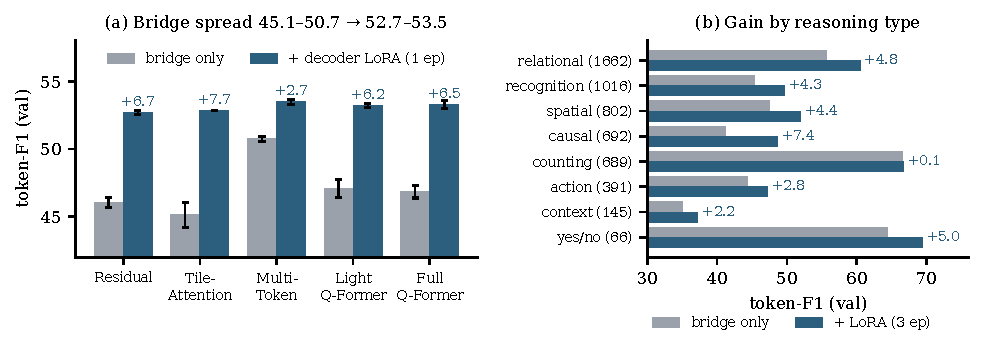
\includegraphics[width=\linewidth]{fig_results}
\caption{(a) Validation F1 against the number of visual tokens (mean $\pm$ std over three
seeds); the circled point is the knee, $g=14$, $k=36$. Horizontal lines: the global-only
model (four seeds) and the same model with a three-epoch decoder LoRA (three seeds).
(b) Validation F1 by reasoning type (number of questions in parentheses): global only and
+ LoRA for seed 42, ViBridge-VQA ($g=14$, $k=36$) without and with a one-epoch decoder LoRA
averaged over three seeds; the numbers give the gain of ViBridge-VQA + LoRA over the
global-only model.}
\label{fig:results}
\end{figure}

Table~\ref{tab:budget} and Fig.~\ref{fig:results}a vary the number of global tokens
$g\in\{8,14\}$ and of local tokens $k\in\{1,9,36,144\}$. The most striking pattern is that
\emph{local tokens matter far more than global ones}. At $g=14$, increasing $k$ from 1 to
144 adds 4.9 F1 and 19.1 CIDEr on the validation split, whereas increasing $g$ from 8 to 14
at a fixed $k$ adds only 0.2--0.6 F1. Accuracy has not saturated within the 144 region
tokens available at our resolution, as each step of $k$ still adds 1.3--2.0 F1, but the gain
per token drops quickly, from 0.07 F1 per token between 23 and 50 tokens to 0.015 between
50 and 158. The budget is therefore a genuine trade-off between accuracy and cost.

Because accuracy grows with every added token, all configurations lie on the Pareto front,
and we select its knee (Section~\ref{sec:budget}). On the validation split, the knee is
$g=14$, $k=36$. Remarkably, the same configuration is the knee for each of the eight
metrics on both validation and test, whether cost is counted in visual tokens or measured
as inference time; with a logarithmic token axis, it remains the knee in 11 of the 16
cases. TOPSIS leads to the same conclusion when accuracy and cost are weighted
equally, using the gains in F1, CIDEr and METEOR as benefits and the added tokens,
inference time, trained parameters and seed variance as costs. Weighting cost more favours
$k=9$, and weighting accuracy more favours $k=144$, but $g=14$, $k=36$ is the only
configuration that stays among the top four for every accuracy weight between 0.3 and 0.7.
In practical terms, it obtains 72\% of the F1 gain of $k=144$ over the global-only
model with 32\% of its visual tokens, and it is the cheapest configuration that reaches the global-only model with a
three-epoch decoder LoRA. Fourteen global tokens are better than eight at every $k$, so we
use $g=14$.

\paragraph{Computational efficiency.}
ViBridge-VQA encodes a single $336\times336$ view per image, which costs 362 GFLOPs and
229\,ms with InternViT-300M on a Tesla P100. The six $448\times448$ tiles and the thumbnail
used by the fine-tuned Vintern-1B cost 2{,}172 GFLOPs and 922\,ms, and give the decoder up to
1{,}792 visual tokens instead of 50. Keeping all 144 local tokens instead of 36 makes evaluation about 17\% slower.

\subsection{Ablation Study}
\label{sec:ablation}



\begin{table}[t]
\centering
\caption{Where the visual tokens come from, with and without decoder adaptation
(validation, $\times100$, mean over three seeds with $\pm$ std for F1; Multi-Token: four
seeds; $^\ast$seed 42 only). Bridge-only models are trained for two epochs; + LoRA is a
rank-16 decoder LoRA trained jointly with the bridge for one epoch (2.16M additional
parameters). Params: trained bridge parameters.}
\label{tab:bridges}
\scriptsize
\setlength{\tabcolsep}{4pt}
\begin{tabular}{lrrrrrr}
\toprule
 & & & \multicolumn{2}{c}{Bridge only} & \multicolumn{2}{c}{+ decoder LoRA} \\
\cmidrule(lr){4-5}\cmidrule(lr){6-7}
Visual tokens from & Tokens & Params & F1 & CIDEr & F1 & CIDEr \\
\midrule
\multicolumn{7}{l}{\emph{Global vector (\texttt{[CLS]})}} \\
\quad Residual & 1 & 4.86M & \pms{46.02}{.36} & 86.48 & \pms{52.69}{.14} & 104.25 \\
\quad Multi-Token & 8 & 7.35M & \pms{50.74}{.17} & 99.07 & \pms{53.47}{.17} & 106.68 \\
\multicolumn{7}{l}{\emph{Learned compression of the patch tokens}} \\
\quad Tile-Attention & 8 & 4.14M & \pms{45.14}{.92} & 84.14 & 52.82$^\ast$ & 104.72$^\ast$ \\
\quad Light Q-Former & 8 & 27.6M & \pms{47.06}{.66} & 88.07 & \pms{53.21}{.14} & 106.26 \\
\quad Full Q-Former & 16 & 69.4M & \pms{46.84}{.47} & 87.74 & \pms{53.29}{.29} & 106.50 \\
\midrule
\multicolumn{7}{l}{\emph{Global vector + pre-trained projector (ViBridge-VQA, $g=14$)}} \\
\quad $k=36$ & 50 & 12.86M & \pms{54.96}{.28} & 113.29 & \pms{\textbf{58.21}}{.16} & \textbf{124.88} \\
\quad $k=144$ & 158 & 12.86M & \pms{\textbf{56.61}}{.04} & \textbf{120.71} & -- & -- \\
\bottomrule
\end{tabular}
\end{table}

\paragraph{Where should the visual tokens come from?}
Table~\ref{tab:bridges} compares three sources of visual tokens for the frozen decoder. The
first group reads only the global \texttt{[CLS]} vector, through a \emph{Residual} bridge
that produces one token or the \emph{Multi-Token} bridge of Eq.~\eqref{eq:bridge}. The
second group learns to compress the patch tokens, either with a \emph{Tile-Attention} bridge
in which eight learned queries attend over the patches, or with a light or full
Q-Former~\cite{li2023blip2}. Without decoder adaptation, the Multi-Token bridge is the best
of these five, and the bridges that compress the patches are 3.7--5.6 F1 lower despite
having up to $9.4\times$ more parameters. Learning a new alignment of the patch tokens from
25k questions thus does not pay off. ViBridge-VQA, which takes the local tokens from the
pre-trained projector instead, improves over the best global-only bridge by 4.2 F1 with
$k=36$ and by 5.9 F1 with $k=144$. The same pooling operation therefore helps when it is
applied to the output of the pre-trained projector, whereas in a preliminary study, pooling
the raw patch tokens through a newly learned projection lost 5.1--13.9 F1 and a
Honeybee-style convolutional abstractor~\cite{cha2024honeybee} remained 0.7 F1 below the
Multi-Token bridge with $2.7\times$ its parameters.

\paragraph{Local tokens and decoder adaptation are complementary.}
A decoder LoRA improves every global-only bridge and brings them within 0.8 F1 of one
another (52.69--53.47), which suggests that the decoder learns to compensate for poor visual
input. Even after this adaptation, all of them remain below ViBridge-VQA with a frozen
decoder. Decoder adaptation is therefore not needed to surpass them, but it is still
useful: in the same one-epoch joint training, it adds 3.3 F1 to ViBridge-VQA, more than the
2.7 F1 it adds to the Multi-Token bridge. Conversely, distilling the projector into
the global-only bridge, at the feature or output level, lowers F1 by 0.3--0.4 points: the
projector's information is best passed as tokens.

\subsection{Analysis by Reasoning Type and Error Analysis}
\label{sec:analysis}

\paragraph{Reasoning types.}
Fig.~\ref{fig:results}b breaks the results down by the reasoning categories of AutoViVQA.
Local tokens help most where the answer depends on what is visible in the image:
recognition (+10.2 F1 over the global-only model), action (+5.4) and spatial (+5.1)
questions. On these categories, ViBridge-VQA with a frozen decoder is also better than the
global-only model with a decoder LoRA. Conversely, decoder adaptation is more useful for
causal and relational questions, whose reference answers are the longest (5.0 and 5.6 words
on average), and for yes/no questions. Adding the LoRA to ViBridge-VQA combines both
strengths: the resulting model is the best in seven of the eight categories, matching the
global-only model with LoRA on causal and relational questions while keeping the large gain
of the local tokens on recognition (58.7 versus 49.7 F1). Local tokens improve what the model
perceives, whereas decoder adaptation improves how it formulates reasoning answers.

\paragraph{Error analysis.}
An analysis of our validation predictions helps explain the low exact-match accuracy of
all systems. Our answers are as long as the references on average (4.3
words), so the gains do not come from changing the answer length. Most predictions (77--81\%) share some, but not all, words with the closest reference: a
correct answer is often phrased differently from all five references. Local tokens turn some of these
partial answers into exact ones and reduce complete failures: compared with the global-only model,
ViBridge-VQA increases the share of predictions with F1 = 1 from 9.8\% to 13.3\% and reduces
the share with no word in common with any reference from 9.6\% to 8.0\% (6.8\% with LoRA).
The remaining failures concentrate on context, recognition, spatial and action questions
(12--18\% without any overlap), i.e., on fine-grained perception, whereas they are rare for
counting, causal and relational questions ($<5\%$), where a partially correct answer is
easier to produce.

\subsection{Generalisation to Other Datasets}
\label{sec:ood}

\begin{table}[t]
\centering
\caption{Zero-shot transfer to Vietnamese VQA datasets not seen during training
($\times100$; about 1{,}000 sampled test questions per sampling seed, 505--519 for ViVQA;
mean over three sampling seeds, $\pm$ std for F1). Vintern-1B reads six tiles and a
thumbnail; the other models are trained on AutoViVQA only (seed 42). Best results per
column are in bold.}
\label{tab:ood}
\scriptsize
\setlength{\tabcolsep}{2.5pt}
\resizebox{\textwidth}{!}{%
\begin{tabular}{lrrrrrrrr}
\toprule
 & \multicolumn{2}{c}{ViTextVQA} & \multicolumn{2}{c}{OpenViVQA} & \multicolumn{2}{c}{ViVQA-X} & \multicolumn{2}{c}{ViVQA} \\
\cmidrule(lr){2-3}\cmidrule(lr){4-5}\cmidrule(lr){6-7}\cmidrule(lr){8-9}
Model & F1 & CIDEr & F1 & CIDEr & F1 & CIDEr & F1 & CIDEr \\
\midrule
Vintern-1B, zero-shot & \pms{32.01}{.31} & \textbf{195.62} & \pms{\textbf{58.40}}{.80} & \textbf{411.63} & \pms{14.52}{.47} & 50.13 & \pms{23.90}{.24} & 78.63 \\
Global only + LoRA, 3 ep. & \pms{3.96}{.09} & 15.64 & \pms{21.56}{.48} & 83.21 & \pms{15.89}{.65} & 42.12 & \pms{31.48}{1.15} & 84.94 \\
\midrule
ViBridge-VQA, $k{=}36$ & \pms{15.14}{.47} & 66.39 & \pms{28.24}{.79} & 128.36 & \pms{24.91}{.14} & 79.51 & \pms{42.68}{1.52} & 171.21 \\
ViBridge-VQA, $k{=}144$ & \pms{\textbf{33.26}}{.67} & 190.30 & \pms{35.89}{.80} & 187.00 & \pms{\textbf{27.89}}{.13} & 92.22 & \pms{\textbf{44.95}}{.90} & \textbf{191.28} \\
ViBridge-VQA, $k{=}36$ + LoRA & \pms{15.39}{.39} & 70.07 & \pms{28.99}{.51} & 130.46 & \pms{27.64}{.11} & \textbf{95.29} & \pms{44.76}{1.21} & 183.60 \\
\bottomrule
\end{tabular}}
\end{table}

Table~\ref{tab:ood} evaluates the models without further training on four Vietnamese VQA
datasets: two scene-text datasets, ViTextVQA~\cite{nguyen2025vitextvqa} and
OpenViVQA~\cite{nguyen2023openvivqa}, and two general-domain ones,
ViVQA-X~\cite{vivqax2025} and ViVQA~\cite{tran2021vivqa}. We include the strongest
global-only model, trained with a three-epoch decoder LoRA, as a reference. Local tokens
change the picture most on scene text, where the global-only model collapses, presumably
because the \texttt{[CLS]} vector cannot convey printed words. On ViTextVQA, F1 rises from 3.96 to 15.14
with 36 local tokens and to 33.26 with 144, slightly above the zero-shot Vintern-1B that
reads six $448\times448$ tiles, although ViBridge-VQA reads a single $336\times336$ view. On
OpenViVQA, whose references are long descriptive sentences, the local tokens narrow the gap
to Vintern-1B, but Vintern-1B remains clearly better.

On the general-domain datasets, ViBridge-VQA outperforms both reference models, by 10.4
(ViVQA-X) and 18.8 (ViVQA) F1 over the zero-shot Vintern-1B with $k=36$. As on AutoViVQA,
the zero-shot model reaches a high recall with long answers (61.2 on ViVQA-X) but a very low
precision (9.1). Adding the decoder LoRA to ViBridge-VQA helps on these general-domain
datasets, bringing $k=36$ close to $k=144$, but barely on scene text. Reading text thus
requires more local tokens, which decoder adaptation cannot replace, consistent with the
token-budget results above.

\subsection{Qualitative Analysis}

\begin{figure}[!tb]
\centering
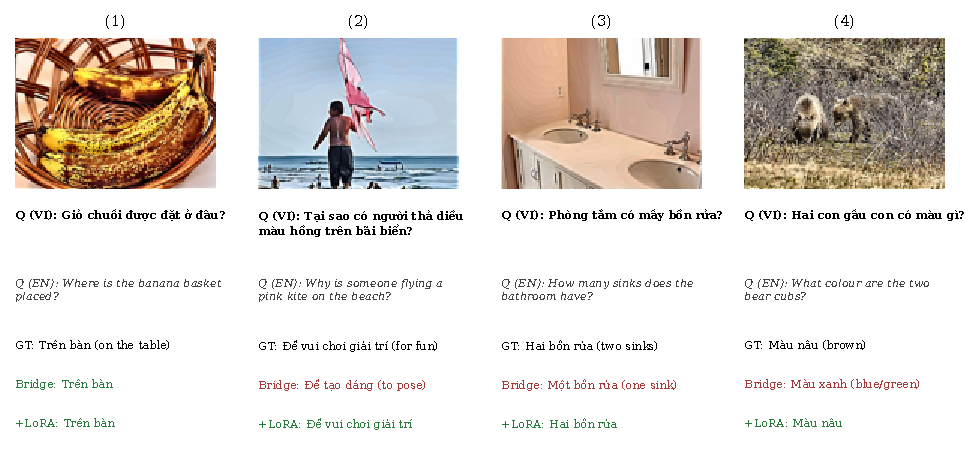
\includegraphics[width=\linewidth]{fig_qualitative}
\caption{Qualitative examples from the AutoViVQA validation set (seed 42). Q: question,
GT: one of the five reference answers, Global: global-only model, +LoRA: the same model with
a three-epoch decoder LoRA, Ours: ViBridge-VQA ($g=14$, $k=36$). Plausible answers are shown
in green and wrong ones in red.}
\label{fig:qual}
\end{figure}

In Examples 1--3 of Fig.~\ref{fig:qual}, only ViBridge-VQA answers correctly, and each
answer depends on a local detail: the brand printed on the
laptop, the canal that identifies Venice, and the water sprayed by the elephant. The
global-only models instead answer ``Apple'', ``Hanoi'' and ``swimming'', which are plausible
for the scene as a whole but wrong for the image. Example~4 shows a typical failure:
ViBridge-VQA describes the scene instead of explaining the purpose of the bus, which both
global-only models infer. This matches the advantage of decoder adaptation on causal questions.

\section{Conclusion}
\label{sec:conclusion}

This work presents \textbf{ViBridge-VQA}, a parameter-efficient adaptation of the
Vietnamese VLM Vintern-1B for generative visual question answering. By keeping the
vision encoder and the language decoder frozen and training only a lightweight
multi-token bridge and a rank-16 decoder LoRA, ViBridge-VQA updates 1.01\% of the
parameters and encodes a single image view. On AutoViVQA it matches the
fine-tuned Vintern-1B on F1, achieves the best generation scores among all
compared systems, and is stable across seeds and splits. Our ablation shows that
the remaining gap is not closed by larger bridges, multi-reference training or
alignment to the original projector, whereas decoder adaptation improves every
bridge and makes them perform almost equally: for a frozen VLM of this size, the
bottleneck lies in the decoder rather than in the visual pathway.

ViBridge-VQA also has limitations. It still trails ViMoE-VQA on precision and F1,
and the fine-tuned Vintern-1B on exact-match accuracy. Because the bridge reads one
global vector of a single view, it is not suited to questions that require
reading scene text\ifoodtext, on which it falls far behind the original
Vintern-1B,\fi{} and it does not improve on counting. The baselines are reported on a different split of
AutoViVQA and were not reproduced in our setting, and our conclusions concern a
frozen 0.5B decoder and may not transfer to larger or fully trainable decoders.
Future work will combine the global-vector bridge with patch-level or
high-resolution tokens for text-heavy questions, and study larger Vietnamese
decoders under the same frozen visual pathway. The code and the grouped split are
available at \url{https://github.com/nguyennn263/modular-vlm-finetune}.

Overall, ViBridge-VQA shows that a strong Vietnamese VQA model can be obtained by
adapting a small fraction of an existing VLM, and that a careful component-wise
analysis indicates where further effort is best spent. We hope this work will
encourage efficient and well-evaluated multimodal models for low-resource
languages.


\begin{credits}
\subsubsection{\ackname} This research is funded by University of Science, VNU-HCM
under grant number CNTT 2025-02.
\end{credits}

\bibliographystyle{splncs04}
\bibliography{references}

\end{document}
